% RQ1
\section{Empirical study}
\label{sec:empiricalstudy}
% Both state of the art tools
% But also commonly used simpler tools
To substantiate further research questions with research data, a empirical study on error detection tools and different configurations is designed. To cover a broad range of configurations (strategies) of these tools, a range of permutations of configurations will be generated for each error detection tool and run on a wide range of datasets with different characteristics and errors. The source code of this framework can be found on GitHub\footnote{\url{\githubsource}}.
~\\Because the source languages of error detection tools differ, a high-level general purpose programming language suits to be used for the framework to connect all the different underlying tools. Together with the fact that it has well-supported libraries for relational data handling, Python\footnote{\url{\pythonsource}} was chosen as the main development language.


\subsection{Setup}
\label{subsec:setup}
First, the setup for the empirical study will be discussed. The basic setup is shown in figure \ref{fig:empiricalsetup}. For each tool in the study, a number of configurations is created, depending on the configurability of the tool. Each configuration in combination with that tool, will be tested on all the available datasets. So a single experiment exists of:
\begin{itemize}
    \item An error detection tool
    \item A tool specific configuration
    \item A target dataset
\end{itemize}

Each experiment will be pushed to the queue of experiments, allowing for retrieving a experiment session without having to rerun all the finished experiments. Incrementally, all the experiment results are pushed into the results database, allowing for the empirical study and further usage with performance prediction and tool ranking. 

\begin{figure}[h]
    \centering
    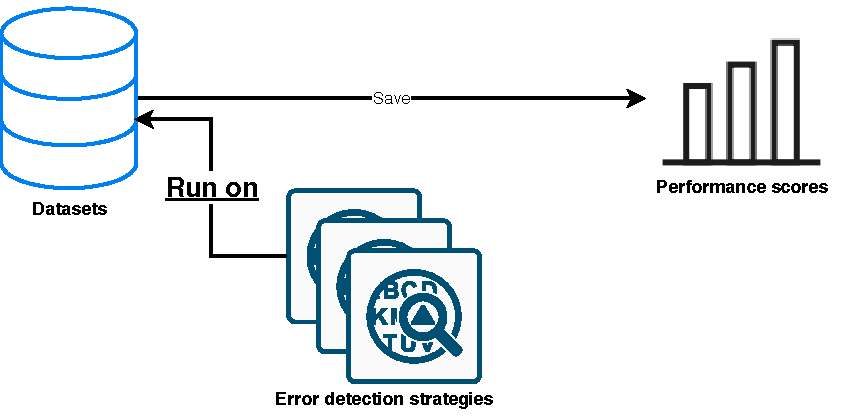
\includegraphics[width=0.9\textwidth]{thesis/Figures/Method/PerformanceEstimation-Experiment.pdf}
    \caption{Setup of the empirical study}
    \label{fig:empiricalsetup}
\end{figure}

% Error detection API to do experiments
\subsection{Error detection framework}
First, a framework for running error detection tools was designed. The purpose of creating a single framework is to have homogeneous in and output for each selected error detection strategies, creating the possibility of running batches of experiments in a structured manner. 
The content and structure of the error detection framework is as follows:
\begin{itemize}[label=\ding{212}]
\item dataset
\item experiment
% \item helpers
%     \begin{itemize}[label=\ding{212}]
%         \item autofd
%         \item autoregex
%     \end{itemize}
\item profiler
\item tool
\item tools
    \begin{itemize}[label=\ding{212}]
        \item ...
        \item see section \ref{subsec:tools}
    \end{itemize}
\end{itemize}

\paragraph{dataset} contains the class for handling datasets for the experiments. It is based upon the work done by \cite{Mahdavi2019-zf} where each dirty dataset has a clean counterpart. Errors can be calculated both cell-wise as well as row-wise. Information about a dataset can be uploaded for later use and metrics like precision, recall and the F1-measure can be calculated from within this class.

\paragraph{experiment} contains the workflow depicted in figure \ref{fig:empiricalsetup}. Objects from this class can create the tool-configuration-dataset triples for the empirical study. Also, it contains the incremental queuing system for execution of experiments, which can be interrupted and resumed at will. Besides the workings shown in figure \ref{fig:empiricalsetup}, this part of the framework supports timeouts of the experiments, to shut down experiments whenever the preconfigured time limit is set. Lastly, it will upload the result metrics, configuration and runtime to a centralized database to further filter and analyze the results.

\paragraph{profiler} contains the elements to profile datasets and predict performance for different tools. This will be further discussed in section \ref{sec:performanceprediction}.

\paragraph{tool} contains the classes for creating error detection tool instances and the base class for tool. The tool creator dynamically finds added tools and is possible to return Tool instances for each error detection tool. Each error detection tool is adjusted to work in similar fashion. It contains an abstract method to run the code, expecting similar input and output for each tool. The tool base class has subprocess functionality to support the timeouts set by the experiment and to run non-Python code. The tool base class also cleans up left over subprocesses whenever timeouts are reached. 

\paragraph{tools} contains each error detection specific implementation of the Tool base class. Only the initialization and the \verb|run| method need to be implemented for each tool work, making it easy to extend this framework. Every tool is implemented in a different submodule. The implemented tools will be further discussed in subsection \ref{subsec:tools}. 



\subsection{Metrics}
\label{subsec:metrics}
To measure the performance of tools on test datasets, metrics of two types can be used. Cell-based and row-based metrics. The difference lies in what is taken as an entity while calculating scores.

\subsubsection{Cell-based metrics}
Cell-based metrics, are metrics that identify each cell in a dataset as a separate entity in the test set. Each cell will be counted as 1 positive or negative. 

\subsubsection{Row-based metrics}
Row-based metrics, are metrics that identify each row in a dataset as a separate entity in the test set. A row could contain multiple errors, but only the whole row is counted as 1 positive or negative.

\subsubsection{Scores}
In the case of error detection, instances are either erroneous (positive) or clean (negative). Because the ground truth of the datasets in section \ref{subsec:datasets} is known, the performance metrics can be calculated directly after the execution of a tool. Precision, recall and the F1-score will be calculated.

\subsubsection{Examples}
To provide visual aid for the different metrics proposed, examples are shown in figures \ref{fig:error_row_wise}. In the figure, the real errors (difference between dirty dataset and the ground truth) are labeled cell-wise by underling and displaying in bold. The "detected" errors by the fictional error detection strategies are shown with a red background. In contrast to the cell-wise detection, the erroneous rows are marked by the black arrows to the left. The "detected" faulty rows are marked by the red arrows on the right.

~\\\textbf{Cell-wise scores} in the examples are as follows. 
\\For figure \ref{subfig:errors_row}, there is a total of 5 real error cells. The detection algorithm marks all 5 errors correctly. So $precision = \frac{5}{5} = 1$, $recall = \frac{5}{5} = 1$ and $F1 = 2 \times \frac{1 \times 1}{1 + 1} = 1$. 
\\For figure \ref{subfig:errors_row_worse}, there are also the same 5 real error cells. The detection algorithm marks only 1 error correctly and 3 more incorrectly. So $precision = \frac{1}{4} = 0.25$, $recall = \frac{1}{5} = 0.2$ and $F1 = 2 \times \frac{0.25 \times 0.2}{0.25 + 0.2} = 0.22$. 

~\\\textbf{Row-wise scores} for the two examples are different than the cell-wise performance scores.
\\For figure \ref{subfig:errors_row}, there is a total of 3 real error rows. The detection algorithm marks all 3 rows correctly. So $precision = \frac{3}{3} = 1$, $recall = \frac{3}{3} = 1$ and $F1 = 2 \times \frac{1 \times 1}{1 + 1} = 1$. 
\\For figure \ref{subfig:errors_row_worse}, there are also the same 3 real error rows. The detection algorithm marks only 1 row correctly and 2 more incorrectly. So $precision = \frac{1}{3} = 0.33$, $recall = \frac{1}{3} = 0.2$ and $F1 = 2 \times \frac{0.33 \times 0.33}{0.33 + 0.33} = 0.33$. 

~\\For this research, \textbf{cell-wise scores} will be used. The goal of error detection in this thesis is to holistically find all different types of errors. Unlike for example duplicate rows, most other errors are defined only for single cells. To also include duplicate rows in the scoring, the complete row is marked as erroneous. The error detection algorithms will be scored accordingly.

\begin{figure}
\centering
    \begin{subfigure}{0.9\textwidth}
        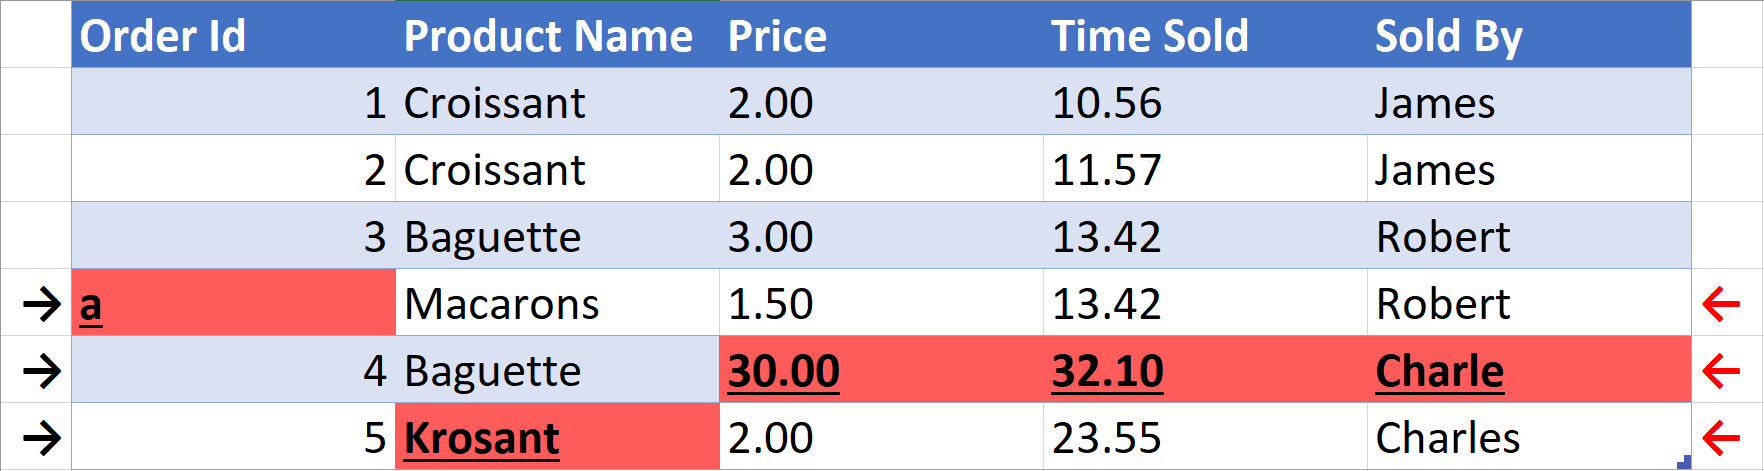
\includegraphics[width=\linewidth]{thesis/Figures/Method/Errors_dataset_F1_row.png}
        \caption{}
        \label{subfig:errors_row}
    \end{subfigure}
    \begin{subfigure}{0.9\textwidth}
        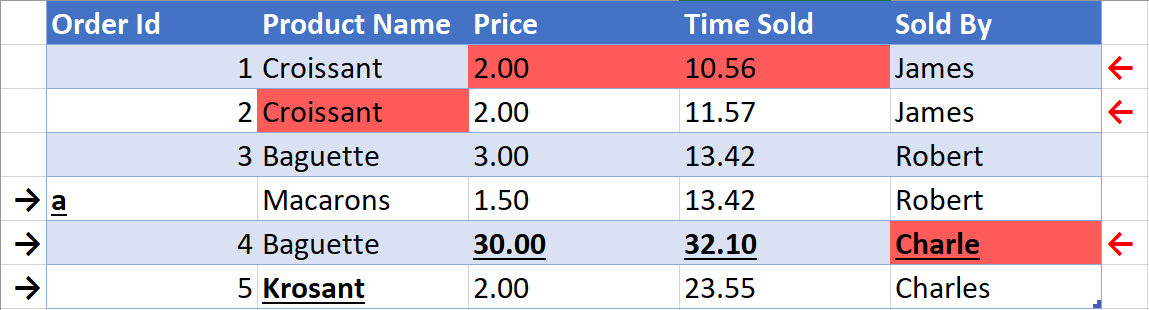
\includegraphics[width=\linewidth]{thesis/Figures/Method/Errors_dataset_Worse_F1_row.png}
        \caption{}
        \label{subfig:errors_row_worse}
    \end{subfigure}
    \caption{Two examples of error detection. Real errors are underlined and bold. Example outputs by error detection methods are marked in red.}
    \label{fig:error_row_wise}
\end{figure}

\begin{table}[]
\centering
\begin{tabular}{l|lll}
\textbf{}    & \textbf{Precision} & \textbf{Recall} & \textbf{F1} \\ \hline
\textbf{(A)} & 1 / 1              & 1 / 1           & 1 / 1       \\
\textbf{(B)} & 0.25 / 0.33        & 0.2 / 0.33      & 0.22 / 0.33
\end{tabular}
\caption{Cell-wise / Row-wise performance score differences for the two examples in figure \ref{fig:error_row_wise}}
\label{tab:cell_vs_row_scores}
\end{table}

\subsection{Datasets}
\label{subsec:datasets}
The datasets selected contained different types of errors, to create a heterogeneous test set to compare the tools and configurations. Errors in a dataset are defined by the difference in the dirty dataset and clean dataset. So only the ground truth makes up an error. Errors can be seen as a transformation of the ground truth to some dirty value. These transformations could specify why the dirty version is wrong. Below are different "error types" that describe errors that have similar transformation between the dirty instance and the ground truth. Of course, there might be overlap in these transformation, as one type of transformation could have the same effect as another type, but these categorizations give an overview of the dataset quality one has to deal with.

\subsubsection{Error types}
The error types are derived from section \ref{subsec:errortypes}, with the addition of the "other errors", which contains errors that cannot be found or described by the default error type categories.

\begin{itemize}
    \item \textit{Outliers:} Values that are erroneous and do not fit in the (column) distribution of the dataset
    \item \textit{Pattern violations:} Values that are erroneous and do not fit in the common pattern of that column (i.e. 2k20 in stead of 2020). Also error values where content and pattern is correct, but with wrong spelling.
    \item \textit{Rule violations:} Also, empty values or missing value placeholders (N/A) that are replaced are supposed to be a real value. Inconsistent abbreviations or references to entities (like states, companies, universities, etc..).
    .\item \textit{Duplicates:} are different tuples, referring to the same real-world entity.
    \item \textit{Other error types:} examples of this type are values that are result of a classification (output) based on the other given columns, but the output is wrong. An error value where the content of the entity is changed, i.e. wrong categories, description or other matters that change the meaning of the underlying value.
\end{itemize}

\subsubsection{Selected datasets}
A summary of the list of datasets used for the empirical study, performance estimation and ranking of error detection strategies can be found below (table \ref{tab:dataset-error-types}). The datasets were taken from published data from the following papers: 
\begin{itemize}
    \item ED2 by \cite{Neutatz2019-aw}
    \item Raha by \cite{Mahdavi2019-zf}
    \item REDS by \cite{Mahdavi2019-pk}
    \item CleanML by \cite{Li2019-ve}
\end{itemize}
The statistics for the used datasets can be found in table \ref{tab:dataset_statistics}.

\begin{table}[]
\begin{adjustbox}{width=\textwidth,center}
\begin{tabular}{|l|c|c|c|c|c|}
\hline
\textbf{Dataset name} & \textbf{Pattern violations} & \textbf{Rule violations} & \textbf{Outliers} & \textbf{Duplicates} & \textbf{Other error types} \\ \hline
\textit{Airbnb}       &                   & \checkmark                                    & \checkmark                             & \checkmark          &                                                 \\ \hline
\textit{Beers}        & \checkmark                                       & \checkmark                                    &                                        &                     &                                                 \\ \hline
\textit{EEG}          &                                                  &                                               & \checkmark                             &                     & \checkmark                                      \\ \hline
\textit{Flights}      & \checkmark                                       & \checkmark                                    &                                        &                     &                                                 \\ \hline
\textit{Hospital}     & \checkmark                                       &                                               &                                        &                     &                                                 \\ \hline
\textit{Marketing} & & \checkmark & & & \checkmark \\ \hline
\textit{Movie}        &                                                  & \checkmark                                    &                                        &  \checkmark                   &                                                 \\ \hline
\textit{Movies}       & \checkmark                                       & \checkmark                                    &                                        &                     & \checkmark                                      \\ \hline
\textit{Rayyan}       & \checkmark                                       & \checkmark                                    &                                        &                     &                                                 \\ \hline
\textit{Restaurant}   & \checkmark                                       & \checkmark                                    &                                        &                     &                                                 \\ \hline
\textit{Restaurants}  & \checkmark                                       &                                               &                                        &                     &                                                 \\ \hline
\textit{Toy}          &                                                  & \checkmark                                    &                                        &                     & \checkmark                                      \\ \hline
\textit{University}   &                                                  & \checkmark                                    &                                        &                     &                                                 \\ \hline
\textit{Uscensus}     &                                                  & \checkmark                                    &                                        &                     & \checkmark                                      \\ \hline
\end{tabular}
\end{adjustbox}
\caption{Table with the datasets used and the common error types present in these datasets}
\label{tab:dataset-error-types}
\end{table}

\paragraph{AirBnb}
This dataset contains 42,492 records on hotels in the top 10 tourist destinations and major US metropolitan areas scraped from Airbnb.com. Each record has 40 attributes including the number of bedrooms, price, location, etc. Demographic and economic attributes were scraped from city-data.com. The classification task is to determine whether the rating of each hotel is 5 or not.
\\(Source: CleanML)

\paragraph{Beers} 
This dataset contains a list of different beers. The attributes are numeric ID's, foreign keys, names, City, state abbreviation, includes amount of ounces \& percentage alcohol.
\\(Source: ED2, REDS, Raha)

\paragraph{EEG}
This is a dataset of 14,980 EEG recordings. Each record has 14 EEG attributes. One of the attributes is a classification task is to predict whether the eye-state is closed or open. In the dirty version of this dataset, some of these predictions are wrong.
\\(Source: CleanML)

\paragraph{Flights}
This dataset contains a flight schedule. Attributes are id, source of data, flight number alphanumeric with dashes, scheduled and actual departure and arrival times in XX:XX a.m. format.
\\(Source: ED2, REDS, Raha)

\paragraph{Hospital}
This source contains a list of hospital experiments. Attributes include ID, hospital names, addresses, measurement types, measurement named, experiment scores and other statistics about the hospital and experiments.
\\(Source: REDS, Raha)

\paragraph{Marketing}
This dataset consists of 8,993 records about household income from a survey. Each record has 14 demographic attributes including sex, education, etc. Another attribute is a classification task is to predict if the annual household income is less than \$25,000.
\\(Source: CleanML)

\paragraph{Movies}
This test set is a collection of popular movies. Attributes of this source are:
Id, Name, Year, Release Date, Director, Creator, Actors, Cast, Language, Country, Duration, RatingValue, RatingCount, ReviewCount, Genre, Filming Locations, Description
\\(Source: ED2, REDS, Raha)

\paragraph{Movie}
Same as movies, but less and different columns
\\(Source: CleanML)

\paragraph{Rayyan}
This dataset contains a set of published articles. The attributes include the title, which journal it was published in, the date, pagination and other information important for citing the articles.
\\(Source: REDS, Raha)

\paragraph{Restaurants}
This source is a list of restaurants. Attributes contain the name, address, phone number, website and other attributes that our commonly found on restaurant review websites (like rating value and price range).
\\(Source: ED2)

\paragraph{Restaurant}
Same idea as "Restaurants", but less columns.
\\(Source: CleanML)

\paragraph{Toy}
Dummy set for testing purposes \& testing for generalizability
\\(Source: REDS, Raha)

\paragraph{University}
This dataset contains 286 records about universities. Each record has 17 attributes including state, university name, SAT scores, etc. It contains a column with a classification task is to predict whether the expenses are greater than 7,000 for each university. This dataset contains inconsistent representations for states and locations.
\\(Source: CleanML)

\paragraph{Uscensus}
This dataset contains 32,561 US Census records for adults. Each record has 14 attributes including age, education, sex, etc. It also contains an attribute with a classification goal of predicting whether the adult earns more than \$50,000. 
\\(Source: CleanML)


\begin{table}
\begin{tabular}{llrrrr}
\toprule
     Dataset & Data quality &   Rows &  Columns &  Number of errors &  Total cells \\
\midrule
      airbnb &       85.4 \% &  18406 &       40 &            107625 &       736240 \\
       beers &       83.5 \% &   2410 &       11 &              4362 &        26510 \\
         eeg &       97.6 \% &  14980 &       15 &              5496 &       224700 \\
     flights &       70.4 \% &   2376 &        7 &              4920 &        16632 \\
    hospital &       97.5 \% &   1000 &       20 &               509 &        20000 \\
   marketing &       78.7 \% &   8993 &       14 &             26815 &       125902 \\
       movie &       63.3 \% &   6531 &        8 &             19174 &        52248 \\
      movies &       98.8 \% &   7390 &       17 &              1501 &       125630 \\
      rayyan &       91.4 \% &   1000 &       11 &               948 &        11000 \\
  restaurant &       99.5 \% &  12007 &       11 &               635 &       132077 \\
 restaurants &       99.9 \% &  28787 &       16 &               565 &       460592 \\
         toy &       77.8 \% &      6 &        3 &                 4 &           18 \\
  university &       97.4 \% &    210 &       18 &               100 &         3780 \\
    uscensus &       99.1 \% &  32561 &       15 &              4262 &       488415 \\
\bottomrule
\end{tabular}
\caption{Dataset statistics}
\label{tab:dataset_statistics}
\end{table}

\subsection{Tools}
\label{subsec:tools}
In this subsection, the tools used in the case study will be discussed. The extensive summary of the workings of the tools can be found in section \ref{chap:background}. The summarized underlying techniques are explained by the common error types that are detectable by the tools as seen in table \ref{tab:tools-error-types}.

\subsubsection{Raha \cite{Mahdavi2019-zf}}
A human-guided error detection system. It selects different preconfigured strategies automatically, based on previously cleaned datasets. Then, it incorporates the \textbf{outputs from various error detection strategies} as a feature vector for the error detection task. Using these feature vectors, it creates clusters of which samples will be labeled in order to reduce user involvement.

\subsubsection{Forbidden Itemsets \cite{Rammelaere2019-ea}}
Applies \textbf{constraint-like method} to detect and repair invalid entries in a dataset. The proposed so-called forbidden itemsets capture unlikely value co-occurrences, similar to denial constraints.

\subsubsection{FAHES \cite{Qahtan2018-te}}
A disguised missing values detector. Whereas most missing value detector focus only on NULL or empty values, this tool takes a different approach. They \textbf{categorize detectable disguised missing values} into five different cases: 1. Out of range data values 2. Outliers 3. String with repeated characters or characters that are next to each other on the used keyboard 4. Values with non-conforming data types 5. Valid values that are randomly distributed within the range of the data and used frequently in the data set.

% \subsubsection{HoloClean \cite{Rekatsinas2017-iw}}
% HoloClean, a data cleaning system that relies on \textbf{statistical learning and inference} to unify a range of data repairing methods. Contributions in this tool include: 1. a compiler that generates a probabilistic model which unifies different signals for repairing a dataset 2. an algorithm that uses Bayesian analysis to prune the domain of the random variables corresponding to noisy cells in the input dataset to systematically tradeoff the scalability and quality of repairs 3. an approximation scheme that relaxes hard integrity constraints to priors over independent random variables.

\subsubsection{ActiveClean \cite{Krishnan2016-rg}}
This tool uses a \textbf{human in the loop to actively learn} which rows are errors. The implementation created uses tf-idf features (frequency–inverse document frequency), created using the scikit-learn \verb|TfidfVectorizer|. The implementation treats each row as a document.

\subsubsection{dBoost \cite{Pit--Claudel2016-dj}}
Outlier Detection in Heterogeneous Datasets using Automatic Tuple Expansion. It uses \textbf{expansion of data tuples using knowledge about the schema and field types}. For example, a timestamp 1424866716 could be expanded into year 2015, Wednesday, etc.. Then outliers are detected based upon these schemas.

\subsubsection{KATARA \cite{Chu2015-fs}}
A \textbf{knowledge base} and crowd powered data cleaning system that, given a table, a knowledge base, and a crowd, interprets table semantics to align it with the knowledge base. KATARA tries to find relations between attributes that have many overlapping values with a type in the knowledge base provided. If with enough confidence a relation is found, the complete set of rows will be checked. If there are mismatches with the knowledge base and the rows, cells will be marked erroneous. 

% \subsubsection{Adapted tools}
% \label{subsubsec:adaptedtools}

\begin{table}[]
\begin{adjustbox}{width=\textwidth,center}
\begin{tabular}{|l|c|c|c|c|}
\hline
\textbf{Tool name} & \textbf{Pattern violations} & \textbf{Rule violations} & \textbf{Outliers} & \textbf{Duplicates} \\ \hline
\textit{ActiveClean}       &  \checkmark & \checkmark &  & \\ \hline
\textit{dBoost}       & \checkmark &  & \checkmark &\\ \hline
\textit{FAHES}       & & \checkmark & &\\ \hline
\textit{Forbidden Itemsets}       & & \checkmark & \checkmark & \checkmark \\ \hline
\textit{KATARA}       & & \checkmark & & \\ \hline
\textit{Raha}       & \checkmark & \checkmark & \checkmark & \checkmark \\ \hline
\end{tabular}
\end{adjustbox}
\caption{Table with the tools used and the common error types that are detectable by the tools}
\label{tab:tools-error-types}
\end{table}

\subsection{Execution \& Analysis}
To answer research question 1; \textit{What is the current state of the art and what is the performance of these tools?}; The different parts from the sections above will be combined. The tools in section \ref{subsec:tools} will be run in selected configurations (tool specific) on all the datasets from section \ref{subsec:datasets}. The main metrics that will be kept are cell-wise precision, recall and F1-score. In a single experiment, a timeout limit is set to filter out tool configuration that do not satisfy runtime needs. The results will be aggregated into showing the best results for a single tool (regardless of its configuration) and the target dataset. This will be shown in a table where the rows represent a single dataset, and each column represents a tool. Such a table will allow quick comparison to see which of the tools performs best for which dataset.
\\Additionaly, these tables can be repeatedly be created with filters (such as no human interaction) or grouping the best scores per tool and dataset based on the selected metrics (i.e. best precision or best F1-score).